\renewcommand{\chaptername}{Chapter}
\chapter{System Architecture and Technical Stack}
\label{chap:architecture-stack}
\vspace{-1cm}

\section{Introduction}

This chapter presents the technical foundation of One Place Chat, focusing on the overall system architecture, database design, and technology stack. We begin with a high-level architectural overview, detail the database schema for both relational and vector storage, present the technologies employed, and conclude with the class diagram illustrating the system's core structure.

\section{Overall System Architecture}

\subsection{High-Level Architecture}

One Place Chat follows a modern three-tier architecture with clear separation of concerns:

\begin{figure}[H]
    \centering
    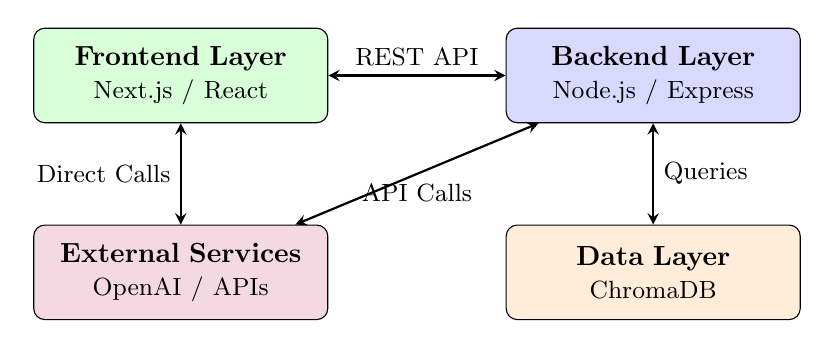
\begin{tikzpicture}[
        node distance=2.5cm,
        box/.style={rectangle, draw, fill=blue!10, text width=3.5cm, align=center, minimum height=1.2cm, rounded corners},
        arrow/.style={->, >=stealth, thick}
    ]
        % Frontend
        \node[box, fill=green!15] (frontend) at (0,0) {\textbf{Frontend Layer}\\{\small Next.js / React}};
        
        % Backend
        \node[box, fill=blue!15] (backend) at (6,0) {\textbf{Backend Layer}\\{\small Node.js / Express}};
        
        % Database
        \node[box, fill=orange!15] (database) at (6,-2.5) {\textbf{Data Layer}\\{\small ChromaDB}};
        
        % External APIs
        \node[box, fill=purple!15] (external) at (0,-2.5) {\textbf{External Services}\\{\small OpenAI / APIs}};
        
        % Arrows
        \draw[arrow, <->] (frontend) -- (backend) node[midway, above, font=\small] {REST API};
        \draw[arrow, <->] (backend) -- (database) node[midway, right, font=\small] {Queries};
        \draw[arrow, <->] (backend) -- (external) node[midway, below, font=\small] {API Calls};
        \draw[arrow, <->] (frontend) -- (external) node[midway, left, font=\small] {Direct Calls};
        
    \end{tikzpicture}
    \caption{Three-Tier System Architecture}
    \label{fig:high-level-architecture}
\end{figure}

\subsection{Component Overview}

The system consists of four primary layers:

\begin{enumerate}
    \item \textbf{Frontend Layer}: User interface built with Next.js and React, handling conversations, knowledge library, and tool management.
    
    \item \textbf{Backend Layer}: Business logic using Node.js and Express, including the conversational engine, semantic tool matching, and API orchestration.
    
    \item \textbf{Data Layer}: ChromaDB vector database storing tools, conversations, and messages with semantic embeddings.
    
    \item \textbf{External Services}: Integration with OpenAI for LLMs and embeddings, plus dynamically discovered third-party APIs.
\end{enumerate}

\section{Database Architecture}

\subsection{Vector Database Strategy}

One Place Chat uses ChromaDB as the primary database, storing all data as vector embeddings with associated metadata:

\begin{figure}[H]
    \centering
    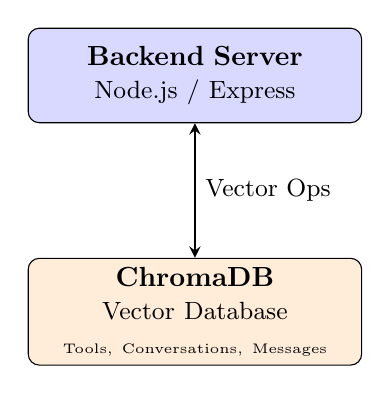
\begin{tikzpicture}[
        node distance=2cm,
        box/.style={rectangle, draw, fill=blue!10, text width=4cm, align=center, minimum height=1.2cm, rounded corners},
        arrow/.style={->, >=stealth, thick}
    ]
        % Backend
        \node[box, fill=blue!15] (backend) at (4,0) {\textbf{Backend Server}\\{\small Node.js / Express}};
        
        % ChromaDB
        \node[box, fill=orange!15] (chromadb) at (4,-3) {\textbf{ChromaDB}\\{\small Vector Database}\\{\tiny Tools, Conversations, Messages}};
        
        % Arrows
        \draw[arrow, <->] (backend) -- (chromadb) node[midway, right, font=\small] {Vector Ops};
        
    \end{tikzpicture}
    \caption{ChromaDB Vector Database Architecture}
    \label{fig:chromadb-architecture}
\end{figure}

\subsection{ChromaDB Collections}

\begin{figure}[H]
    \centering
    \includegraphics[width=0.9\linewidth]{screens/diagramme.png}
    \caption{ChromaDB Collection Schema and Relationships}
    \label{fig:chromadb-schema}
\end{figure}

\subsubsection{Collection Descriptions}

\textbf{Users Collection:} Stores user profiles with unique identifiers, email addresses, display names, and roles. Each user record includes timestamps for account creation and last login activity.

\textbf{Generated Tools Collection:} Contains API tool definitions automatically generated from OpenAPI specifications. Each tool includes a 1536-dimensional embedding vector from OpenAI's \texttt{text-embedding-ada-002} model, enabling semantic similarity search. The document field stores the complete MCPTool definition including name, description, HTTP method, and endpoint path.

\textbf{Conversations Collection:} Manages conversation contexts with references to the owning user. Each conversation stores its embedding for similarity-based retrieval, the complete conversation context as JSON, title, message count, and activity timestamps.

\textbf{Messages Collection:} Stores individual messages belonging to conversations. Each message contains its role (user, assistant, or system), content, timestamp, and an embedding for fine-grained semantic search within conversation history.

\subsubsection{Collection Relationships}

The collections are linked through the following relationships:
\begin{itemize}
    \item \textbf{Users $\rightarrow$ Conversations}: One user can own multiple conversations (1:N relationship)
    \item \textbf{Conversations $\rightarrow$ Messages}: One conversation contains multiple messages
\end{itemize}

\section{System Class Diagram}

The following class diagram illustrates the main backend components and their relationships:

\begin{figure}[H]
    \centering
    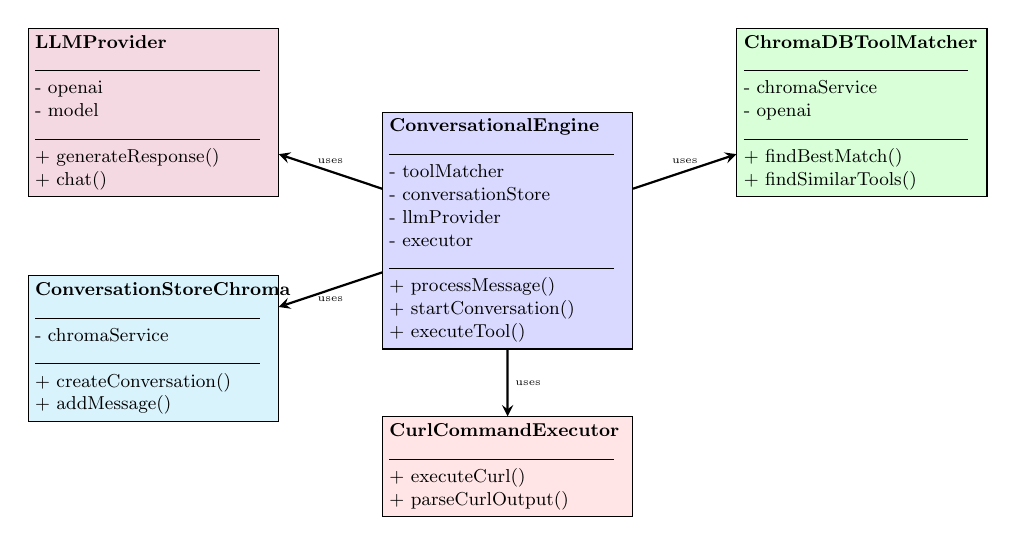
\begin{tikzpicture}[scale=0.75, transform shape]
        % Define styles
        \tikzstyle{class}=[rectangle, draw, text width=4cm, align=left, font=\small]
        \tikzstyle{arrow}=[->, >=stealth, thick]
        
        % ConversationalEngine (center)
        \node[class, fill=blue!15] (engine) at (0,0) {
            \textbf{ConversationalEngine}\\
            \rule{3.8cm}{0.4pt}\\
            - toolMatcher\\
            - conversationStore\\
            - llmProvider\\
            - executor\\
            \rule{3.8cm}{0.4pt}\\
            + processMessage()\\
            + startConversation()\\
            + executeTool()
        };
        
        % ChromaDBToolMatcher
        \node[class, fill=green!15] (matcher) at (6,2) {
            \textbf{ChromaDBToolMatcher}\\
            \rule{3.8cm}{0.4pt}\\
            - chromaService\\
            - openai\\
            \rule{3.8cm}{0.4pt}\\
            + findBestMatch()\\
            + findSimilarTools()
        };
        
        % LLMProvider
        \node[class, fill=purple!15] (llm) at (-6,2) {
            \textbf{LLMProvider}\\
            \rule{3.8cm}{0.4pt}\\
            - openai\\
            - model\\
            \rule{3.8cm}{0.4pt}\\
            + generateResponse()\\
            + chat()
        };
        
        % ConversationStore
        \node[class, fill=cyan!15] (store) at (-6,-2) {
            \textbf{ConversationStoreChroma}\\
            \rule{3.8cm}{0.4pt}\\
            - chromaService\\
            \rule{3.8cm}{0.4pt}\\
            + createConversation()\\
            + addMessage()
        };
        
        % CurlCommandExecutor
        \node[class, fill=red!10] (curl) at (0,-4) {
            \textbf{CurlCommandExecutor}\\
            \rule{3.8cm}{0.4pt}\\
            + executeCurl()\\
            + parseCurlOutput()
        };
        
        % Arrows
        \draw[arrow] (engine) -- (matcher) node[midway, above, font=\tiny] {uses};
        \draw[arrow] (engine) -- (llm) node[midway, above, font=\tiny] {uses};
        \draw[arrow] (engine) -- (store) node[midway, below, font=\tiny] {uses};
        \draw[arrow] (engine) -- (curl) node[midway, right, font=\tiny] {uses};


        
    \end{tikzpicture}
    \caption{Backend System Class Diagram}
    \label{fig:class-diagram}
\end{figure}

\subsection{Class Responsibilities}

\begin{itemize}
    \item \textbf{ConversationalEngine}: Main orchestrator coordinating tool matching, parameter extraction, LLM interactions, and API execution.
    
    \item \textbf{ChromaDBToolMatcher}: Performs semantic matching between user queries and available tools using OpenAI embeddings.
    
    \item \textbf{ChromaDBService}: Low-level client for ChromaDB operations including embedding storage and similarity search.
    
    \item \textbf{LLMProvider}: Abstraction layer for large language model interactions, supporting OpenAI GPT models.
    
    \item \textbf{ConversationStoreChroma}: Manages conversation persistence and message history in ChromaDB.
    
    \item \textbf{CurlCommandExecutor}: Generates and executes cURL commands to call external APIs.
\end{itemize}

\section{Conclusion}

The One Place Chat architecture combines a modern three-tier design with a dual-database strategy optimized for both structured data management and AI-powered semantic search. The technology stack leverages industry-standard tools while the class structure ensures maintainability through clear separation of concerns. This foundation enables the system to automatically integrate new APIs, understand natural language queries through vector similarity, and deliver intelligent responses reliably.
